%%%%%%%%%%%%%%%%%%%% book.tex %%%%%%%%%%%%%%%%%%%%%%%%%%%%%
%
% sample root file for the chapters of your "monograph"
%
% Use this file as a template for your own input.
%
%%%%%%%%%%%%%%%% Springer-Verlag %%%%%%%%%%%%%%%%%%%%%%%%%%


% RECOMMENDED %%%%%%%%%%%%%%%%%%%%%%%%%%%%%%%%%%%%%%%%%%%%%%%%%%%
\documentclass[graybox,envcountchap,sectrefs]{svmono}

% choose options for [] as required from the list
% in the Reference Guide

%\usepackage{mathptmx}
%\usepackage{helvet}
%\usepackage{courier}
%
\usepackage{type1cm}         

\usepackage{makeidx}         % allows index generation
\usepackage{graphicx}        % standard LaTeX graphics tool
                             % when including figure files
\usepackage{multicol}        % used for the two-column index
\usepackage[bottom]{footmisc}% places footnotes at page bottom

\usepackage{newtxtext}       % 
\usepackage[varvw]{newtxmath}       % selects Times Roman as basic font

% see the list of further useful packages
% in the Reference Guide

% KOMA setup
\usepackage{scrlayer-scrpage}
\pagestyle{scrheadings}
%\addtokomafont{pagenumber}{\oldstylenums}
\clearscrheadfoot %% <-----
\lehead{\headmark}% left even head <===================================
\rehead[\pagemark]{\pagemark}
\lohead[\pagemark]{\pagemark}
\rohead{\headmark}% right odd head <===================================

% Change font
%\usepackage{mathptmx}

% Character set
\usepackage{cmap}
\usepackage[utf8]{inputenc}
% 20190927: fontenc-T1 causes problems with ttfamily, causing
% lstinline to be incorrectly set!
\usepackage[T1]{fontenc} % ensure that all the characters in characterSets.tex prints
\usepackage{upquote} % \textcent
\usepackage{pifont} % add \ding, http://ctan.org/pkg/pifont
\renewcommand{\Re}{\mathbb{R}}
\newcommand{\Nat}[0]{\mathbb{N}}
\newcommand{\Int}[0]{\mathbb{Z}}

% for formatting (large) numbers
\usepackage{numprint}
\npthousandsep{\,}


% Figures
%\usepackage{graphicx} % springer has it
\graphicspath{ {./figures/} {../figures/} }

% % % A background text to prevent wide distribution
% \usepackage{draftwatermark}
% \SetWatermarkText{DRAFT}
% \SetWatermarkScale{6}
% %\SetWatermarkScale{1.5}  %mathptmx
% \SetWatermarkLightness{.95}

\renewcommand{\floatpagefraction}{.8}%
\setlength{\textfloatsep}{5pt plus 1.0pt minus 1.0pt}
\setlength{\floatsep}{5pt plus 1.0pt minus 1.0pt}
\setlength{\intextsep}{5pt plus 1.0pt minus 1.0pt}

% force floats to [H] - here definitely
%\usepackage{float}
%\floatplacement{figure}{!h}
%\floatplacement{table}{!h}

% paragraph indentation is stupid
\setlength\parindent{0pt}
\setlength{\parskip}{1em}

% Globally defined colors
%\usepackage[table,x11names]{xcolor} % springer has it
\definecolor{alternateKeywordsColor}{rgb}{0.13,1,0.13}
\definecolor{keywordsColor}{rgb}{0.13,0.13,1}
%\definecolor{commentsColor}{rgb}{0,0.5,0}
\definecolor{commentsColor}{rgb}{0,0.5,0}
%\definecolor{stringsColor}{rgb}{0.9,0,0}
\definecolor{stringsColor}{rgb}{0,0,0.5}
\definecolor{light-gray}{gray}{0.95}
\definecolor{codeLineHighlight}{named}{SlateGray1}
%\definecolor{codeLineHighlight}{rgb}{0.975,0.975,0.975}
\definecolor{syntaxColor}{rgb}{0,.45,0}

\definecolor{headerRowColor}{rgb}{0.85,0.85,0.85}
\definecolor{subHeaderRowColor}{rgb}{0.95,0.95,0.95}
\definecolor{oddRowColor}{rgb}{0.95,0.95,0.95}
\definecolor{evenRowColor}{rgb}{1,1,1}

\definecolor{verb}{rgb}{0,0.75,0}
\definecolor{noun}{rgb}{0,0,0.75}

% add check- and crossmarks, http://ctan.org/pkg/pifont
\newcommand{\cmark}{{\color{green}\ding{51}}}%
\newcommand{\xmark}{{\color{red}\ding{55}}}%

% Add better time and date support
\usepackage{datetime2}

% Extra math stuff
%\usepackage{amsmath,amssymb} % Removed for springer

% Typeset chess
\usepackage{skak}

% clickable url
\usepackage{url}

% figures
\usepackage{subfigure}

% Footnotes below floats
%\usepackage[multiple,bottom]{footmisc} % remove for springer

% Avoid pagebreaks in footnotes
\interfootnotelinepenalty=10000

%%%%%% fncychap only works with default setup!!!!! Missing section number!!!!
%Fancy chapter headings
%\usepackage{fncychap}
%%%%%% titlesec no longer works (2019)!!!!! Missing section number!!!!
%\usepackage[rm]{titlesec}
%\usepackage[sf,sl,outermarks]{titlesec}
% \definecolor{gray75}{gray}{0.75}
% \newcommand{\hsp}{\hspace{20pt}}
% \titleformat{\chapter}[hang]{\Huge\bfseries}{\thechapter\hsp\textcolor{gray75}{|}\hsp}{0pt}{\Huge\bfseries}

% Clickable table of content
\usepackage[pdfpagelabels]{hyperref}
%\usepackage{multirow}
\usepackage{makecell}

% Include label name in ref
\usepackage[noabbrev,capitalize]{cleveref}
\newcommand{\creflastconjunction}{, and\nobreakspace~}
\Crefformat{tcb@cnt@codeNOutput}{Listing~#2#1#3}
\crefformat{tcb@cnt@codeNOutput}{Listing~#2#1#3}
\crefrangeformat{tcb@cnt@codeNOutput}{Listing~#3#1#4\nobreakdash--#5#2#6}
\Crefrangeformat{tcb@cnt@codeNOutput}{Listing~#3#1#4\nobreakdash--#5#2#6}
\crefmultiformat{tcb@cnt@codeNOutput}{Listing~#2#1#3}{ and~#2#1#3}{, #2#1#3}{\creflastconjunction#2#1#3}
\Crefmultiformat{tcb@cnt@codeNOutput}{Listing~#2#1#3}{ and~#2#1#3}{, #2#1#3}{\creflastconjunction#2#1#3}
\crefrangeformat{table}{Table~#3#1#4\nobreakdash--#5#2#6}
\Crefrangeformat{table}{Table~#3#1#4\nobreakdash--#5#2#6}
\crefrangeformat{part}{Part~#3#1#4\nobreakdash--#5#2#6}
\Crefrangeformat{part}{Part~#3#1#4\nobreakdash--#5#2#6}

% paragraphs in tables
\usepackage{tabularx}
\newcolumntype{Y}{>{\raggedright\arraybackslash}X}
\usepackage{pdflscape}
\usepackage{afterpage}
\usepackage{capt-of}
\usepackage{longtable}
\usepackage{makecell}

% formatting lists
\usepackage{enumitem}
%\setlist[description]{leftmargin=0pt,labelindent=0pt,itemindent=0pt}
%\setlist[description]{itemindent=-\leftmargin}

% latex comment environment
\usepackage{comment}

% UML
\usepackage[school,simplified]{pgf-umlcd}
\renewcommand{\umltextcolor}{black} 
\renewcommand{\umlfillcolor}{black!5!white}
\renewcommand{\umldrawcolor}{teal}

% List of indices
\usepackage{marginnote}
\usepackage{xstring}
\usepackage{makeidx}
\usepackage{marginfix} % fixes marginpar location problem in 2 -page mode.
%\newcommand{\idxs}[1]{\marginpar{$\cdot$~\parbox[t]{\linewidth}{\raggedright \expandarg\IfSubStr{#1}{@}{\StrBehind{#1}{@}}{#1}}}\index{#1}} % The parbox is too wide, since the line also includes cdot-space
\newcommand{\idxs}[1]{\marginnote{%$\cdot$~\parbox[t]{\linewidth}{\raggedright \expandarg\IfSubStr{#1}{@}{\StrBehind{#1}{@}}{#1}}
                                                                              }\index{#1}} % The parbox is too wide, since the line also includes cdot-space
\newcommand{\idxss}[1]{\index{#1}}
% Define a new command idx with an optional parameter, which if given is the key to the index
\makeatletter
\def\idx{\@ifnextchar[{\@with}{\@without}}
\def\@with[#1]#2{\emph{#2}\idxs{#1}}
\def\@without#1{\emph{#1}\idxs{#1}}
\makeatother
%\newcommand{\idx}[1]{\emph{#1}\idxs{#1}}
\newcommand{\keyword}[1]{{\lstinline[language=fsharp]|#1|}}
\newcommand{\lexeme}[1]{\mbox{``\lstinline[language=fsharp]{#1}''}}
\makeindex

% display tree like structures
\usepackage{qtree}

% We frame all listings and problems
\usepackage{tcolorbox}
\tcbuselibrary{listings}
\tcbuselibrary{raster}
\tcbset{%
  colframe=teal, %PaleGreen1!45!black,
  %coltitle=black,
  fonttitle=\bfseries, 
  leftrule=3mm,
  sharp corners=downhill,
  colback=black!5!white,
  left=1mm,
  top=0mm,
  right=1mm,
  bottom=0mm,
  middle=1mm,
  arc=2mm,
}
%\newtcolorbox[auto counter, number within=chapter]{task}[1][]{% % removed for springer
%  title=\textbf{Problem~\thetcbcounter},
%  colframe=DeepSkyBlue1, %green!30!blue,
%  #1}

\newenvironment{objectives}
{
   \begin{overview}{Chapter points}%
   %\par\noindent\rule{\textwidth}{0.4pt}
}{ 
   \end{overview}%
%   \par\noindent\rule{\textwidth}{0.4pt}
}


\newtcolorbox[auto counter, number within=chapter]{task}[2][]{% % removed for springer
  title=\textbf{Problem~\thetcbcounter},
  colframe=DeepSkyBlue1, %green!30!blue,
  label=#2,
  #1}
\newcommand{\src}{src}
\newtcolorbox[auto counter, number within=chapter]{codeNOutput}[2][]{%
  title=\textbf{Listing~\thetcbcounter#2},
  #1}

%% lstlisting stuff
\usepackage{listings} 
\def\lstfs#1{\mbox{\lstinline{{#1}}}}
% Get counters from references for firstnumber references in lstinputlisting
\usepackage{refcount}
\newcounter{lstFrom}
\newcounter{lstTo}
% Example: 
% \setcounterref{lstFrom}{dynamicScopeTracing:a1}
% \setcounterref{lstTo}{dynamicScopeTracing:a2}
% \lstinputlisting[firstline=\thelstFrom,lastline=\thelstTo,escapechar=|]{\src/dynamicScopeTracing.fsx}

%%%%%%% Latest version of listing package is incompatible with lstlinebdgrd :(
% \usepackage{lstlinebgrd}

%%%% Attempt to temporary fix according https://tex.stackexchange.com/questions/451532/recent-issues-with-lstlinebgrd-package-with-listings-after-the-latters-updates
\makeatletter
\let\old@lstKV@SwitchCases\lstKV@SwitchCases
\def\lstKV@SwitchCases#1#2#3{}
\makeatother
\usepackage{lstlinebgrd}
\makeatletter
\let\lstKV@SwitchCases\old@lstKV@SwitchCases

\lst@Key{numbers}{none}{%
    \def\lst@PlaceNumber{\lst@linebgrd}%
    \lstKV@SwitchCases{#1}%
    {none:\\%
     left:\def\lst@PlaceNumber{\llap{\normalfont
                \lst@numberstyle{\thelstnumber}\kern\lst@numbersep}\lst@linebgrd}\\%
     right:\def\lst@PlaceNumber{\rlap{\normalfont
                \kern\linewidth \kern\lst@numbersep
                \lst@numberstyle{\thelstnumber}}\lst@linebgrd}%
    }{\PackageError{Listings}{Numbers #1 unknown}\@ehc}}
\makeatother
%%%% Attempt to temporary fix according https://tex.stackexchange.com/questions/451532/recent-issues-with-lstlinebgrd-package-with-listings-after-the-latters-updates

\makeatletter
%The following sets the box compatible with tcolorbox setup
\def\lst@linebgrdcolor{\color{black!5!white}}
\def\lst@linebgrdsep{1em}
\def\lst@linebackgroundwidth{1em}
\def\lst@linebackgroundhighlight{\color{codeLineHighlight}}
\renewcommand{\lst@linebgrd}{%
  \ifx\lst@linebgrdcolor\empty
  \else
    \rlap{
       \lst@basicstyle\color{black!5!white} % tcolorbox background color
       \lst@linebgrdcolor{
          \kern-\dimexpr\lst@linebgrdsep\relax
          \lst@linebgrdcmd{\lst@linebgrdwidth}{\lst@linebgrdheight}{\lst@linebgrddepth}
       }
    }
  \fi
}
% Highlight a range of lines with green. Use \getrefnumber{label} for refs
\newcommand{\highlightRange}[2]{\ifnum\value{lstnumber}>\numexpr#1-1\ifnum\value{lstnumber}<\numexpr1+#2\lst@linebackgroundhighlight\fi\fi}
% \highlight conflicts with skak. Just rewriting, wonder what breaks in skak
\renewcommand{\highlight}[1]{\ifnum\value{lstnumber}=#1\lst@linebackgroundhighlight\fi}

\renewcommand{\highlightRange}[2]{}
\renewcommand{\highlight}[1]{}

%%%%%%% Latest version of listing package is incompatible with lstlinebdgrd :(

% To use verbatimwrite to write listing to file, e.g., in conjunction with ebnfs
\usepackage{moreverb} 

\lstdefinelanguage{fsharp}{%
  keywords={abstract, and, as, assert, base, begin, class, default, delegate, do, done, downcast, downto, elif, else, end, exception, extern, false, finally, for, fun, function, global, if, in, inherit, inline, interface, internal, lazy, let, match, member, module, mutable, namespace, new, null, of, open, or, override, private, public, rec, return, sig, static, struct, then, to, true, try, type, upcast, use, val, void, when, while, with, yield},
  morekeywords={atomic, break, checked, component, const, constraint, constructor, continue, eager, fixed, fori, functor, include, measure, method, mixin, object, parallel, params, process, protected, pure, recursive, sealed, tailcall, trait, virtual, volatile},
  otherkeywords={ let!, return!, do!, yield!, use!},
  keywordstyle=\color{keywordsColor},
  % sensitive=true,
  basicstyle=\ttfamily\lst@ifdisplaystyle\footnotesize\fi, % make font small for listings but not for lstinline
  breaklines=true,
  breakatwhitespace=true
  showstringspaces=false,
  morecomment=[l][\color{commentsColor}]{///},
  morecomment=[l][\color{commentsColor}]{//},
  morecomment=[n][\color{commentsColor}]{(*}{*)},
  morecomment=[is][\color{white}]{(*//}{*)},
  morestring=[b]",
  literate={`}{\`}1,
  stringstyle=\color{stringsColor},
  showspaces=true,
  numbers=left,
  numbersep=1.5pt,
  numberstyle=\scriptsize\color{white},
  % aboveskip=0pt, 
  % belowskip=0pt,
  % resetmargins=true,
  % captionpos=b,
  backgroundcolor=\color{black!5!white},
}


\lstdefinelanguage{syntax}{%
  classoffset=0,
  keywords={abstract, and, as, assert, base, begin, class, default, delegate, do, done, downcast, downto, elif, else, end, exception, extern, false, finally, for, fun, function, global, if, in, inherit, inline, interface, internal, lazy, let, match, member, module, mutable, namespace, new, null, of, open, or, override, private, public, rec, return, sig, static, struct, then, to, true, try, type, upcast, use, val, void, when, while, with, yield, atomic, break, checked, component, const, constraint, constructor, continue, eager, fixed, fori, functor, include, measure, method, mixin, object, parallel, params, process, protected, pure, recursive, sealed, tailcall, trait, virtual, volatile, let!, return!, do!, yield!, use!},
  keywordstyle=\color{keywordsColor},
  % classoffset=1,
  % morekeywords={ident, expr, arg, format-string},
  % keywordstyle=\color{syntaxColor},
  % classoffset=0,
  otherkeywords={},
  basicstyle=\ttfamily\lst@ifdisplaystyle\footnotesize\fi, % make font small for listings but not for lstinline
  breaklines=true,
  breakatwhitespace=true
  showstringspaces=false,
  classoffset=0,
  morecomment=[l][\color{commentsColor}]{////},
  literate={`}{\`}1 {\{*}{{{\color{syntaxColor}\{}}}1 {*\}}{{{\color{syntaxColor}\}}}}1 {[*}{{{\color{syntaxColor}[}}}1  {*]}{{{\color{syntaxColor}]}}}1 {(*}{{{\color{syntaxColor}(}}}1  {*)}{{{\color{syntaxColor})}}}1 {|*}{{{\color{syntaxColor}|}}}1, % {etc*}{{{\color{syntaxColor}...}}}3,
  moredelim  = **[is][\processmydelims]{<*}{*>}, % delete delimiters, typeset keywords. Don't know how to avoid the last...
  showspaces=true,
  numbers=left,
  numbersep=1.5pt,
  numberstyle=\scriptsize\color{white},
  backgroundcolor=\color{black!5!white},
}
%Tweek of deliminter and literate: https://tex.stackexchange.com/questions/203263/listings-package-custom-language-delimiter-match-left-side
\newcommand\processmydelimsend{}
\newcommand\processmydelims{%
  \renewcommand\processmydelimsend{\textcolor{syntaxColor}{>}\egroup}%
  \bgroup\color{syntaxColor}<\aftergroup\processmydelimsend%
}
% \makeatletter
% \newcommand\processhash{%
%   \ifnum\lst@mode=\lst@Pmode%
%     \bfseries%
%   \fi
%   \#%
% }
% \makeatother


\lstdefinelanguage{ebnf}{%
  keywords={},
  morekeywords={},
  otherkeywords={},
  keywordstyle=\color{keywordsColor},
  % sensitive=true,
  basicstyle=\fontfamily{pcr}\selectfont\lst@ifdisplaystyle\footnotesize\fi, 
  breaklines=true,
  breakatwhitespace=true
  morecomment=[s][\color{commentsColor}]{(*}{*)},
  morestring=[b]",
  morestring=[b]',
  alsoletter={\\},
  showstringspaces=false,
  % stringstyle=\color{stringsColor},
  % aboveskip=0pt, 
  % belowskip=0pt,
  % resetmargins=true,
  % captionpos=b,
  % backgroundcolor=\color{blue!10!white},
}
\lstdefinelanguage{console}{%
  keywords={},
  morekeywords={},
  otherkeywords={},
  basicstyle=\ttfamily\lst@ifdisplaystyle\footnotesize\fi, 
  breaklines=true,
  showstringspaces=false,
  % aboveskip=0pt,
  % belowskip=0pt,
  % resetmargins=true,
  % captionpos=b,
  % backgroundcolor=\color{green!10!white},
}
%\lstset{language=fsharp, frame=single}
\lstset{language=fsharp}
\makeatletter
\def\lst@visiblespace{ }
\makeatother

% input .fsx and .out listings from \src and display as code and result in same figure
% #1 = optional further arguments for lstinputlisting
% #2 = filename without suffix, and label
% #3 = caption
\newtcbinputlisting[use counter from=codeNOutput]{\fs}[3][]{%
  top=-5pt,
  bottom=-5pt,
  left=-2pt,
  right=-2pt,
  listing file={src/#2.fsx},
  listing and comment,
  listing options={language=fsharp,escapechar=§,#1},
  float,
  title=\textbf{Listing \thetcbcounter} {#2.fsx:\\#3},
  %title=\textbf{Listing \thetcbcounter} {#3},
  label={#2},
  comment={\lstinputlisting[language=console]{\src/#2.out}}
}

% dispaly fsharp code \src
% #1 = optional further arguments for lstinputlisting
% #2 = filename
% #3 = label
% #4 = caption
\newtcbinputlisting[use counter from=codeNOutput]{\fsharp}[4][]{%
  top=-5pt,
  bottom=-5pt,
  left=-2pt,
  right=-2pt,
  listing file={\src/#2},
  listing only,
  listing options={language=fsharp,escapechar=§,#1},
  float,
  title=\textbf{Listing \thetcbcounter} {#2:\\#4},
  %title=\textbf{Listing \thetcbcounter} {#4},
  label={#3},
}

% dispaly console file \src
% #1 = optional further arguments for lstinputlisting
% #2 = filename
% #3 = label
% #4 = caption
\newtcbinputlisting[use counter from=codeNOutput]{\console}[4][]{%
  top=-5pt,
  bottom=-5pt,
  left=-2pt,
  right=-2pt,
  listing file={\src/#2},
  listing only,
  listing options={language=console,escapechar=§,#1},
  float,
  title=\textbf{Listing \thetcbcounter} {#2:\\#4},
  %title=\textbf{Listing \thetcbcounter} {#4},
  label={#3},
}

\newtcbinputlisting[use counter from=codeNOutput]{\fsCode}[4]{%
  top=-5pt,
  bottom=-5pt,
  left=-2pt,
  right=-2pt,
  listing file={src/#1.fsx},
  listing only,
  listing options={language=fsharp,escapechar=§,#4},
  float,
  title=\textbf{Listing \thetcbcounter} {#1.fsx:\\#3},
  %title=\textbf{Listing \thetcbcounter} {#3},
  label={#2},
}

\newtcbinputlisting[use counter from=codeNOutput]{\fsSignature}[4]{%
  top=-5pt,
  bottom=-5pt,
  left=-2pt,
  right=-2pt,
  listing file={src/#1.fsi},
  listing only,
  listing options={language=fsharp,escapechar=§,#4},
  float,
  title=\textbf{Listing \thetcbcounter} {#1.fsi:\\#3},
  %title=\textbf{Listing \thetcbcounter} {#3},
  label={#2},
}
\newtcbinputlisting[use counter from=codeNOutput]{\fsImplementation}[4]{%
  top=-5pt,
  bottom=-5pt,
  left=-2pt,
  right=-2pt,
  listing file={src/#1.fs},
  listing only,
  listing options={language=fsharp,escapechar=§,#4},
  float,
  title=\textbf{Listing \thetcbcounter} {#1.fs:\\#3},
  %title=\textbf{Listing \thetcbcounter} {#3},
  label={#2},
}

% dispaly output file .out from \src
% #1 = optional further arguments for lstinputlisting
% #2 = filename without suffix, and label
% #3 = caption
\newtcbinputlisting[use counter from=codeNOutput]{\fsOutput}[3][]{%
  top=-5pt,
  bottom=-5pt,
  left=-2pt,
  right=-2pt,
  listing file={src/#2.out},
  listing only,
  listing options={language=console,escapechar=§,#1},
  float,
  title=\textbf{Listing \thetcbcounter}: {#3},
  label={#2},
}

% dispaly output file .out from \src
% #1 = optional further arguments for lstinputlisting
% #2 = filename without suffix, and label
% #3 = caption
\newtcbinputlisting[use counter from=codeNOutput]{\fsOutputNF}[3][]{%
  top=-5pt,
  bottom=-5pt,
  left=-2pt,
  right=-2pt,
  listing file={src/#2.out},
  listing only,
  listing options={language=console,escapechar=§,#1},
  % float,
  title=\textbf{Listing \thetcbcounter}: {#3},
  label={#2},
}

% dispaly output file .out from \src as an element in tabularx
% #1 = optional further arguments for lstinputlisting
% #2 = filename without suffix, and label
% #3 = caption
\newtcbinputlisting[use counter from=codeNOutput]{\fsOutputTabx}[3][]{%
  top=-5pt,
  bottom=-5pt,
  left=-2pt,
  right=-2pt,
  listing file={src/#2.out},
  listing only,
  width=\hsize,
  box align=top,
  listing options={language=console,escapechar=§,aboveskip=0pt,belowskip=0pt,emptylines=0,#1},
  float,
  title=\textbf{Listing \thetcbcounter}: {#3},
  label={#2},
}

% dispaly ebnf file, no label
% #1 = optional further arguments for lstinputlisting
% #2 = filename
% #3 = caption
\newtcbinputlisting[use counter from=codeNOutput]{\ebnf}[3][]{%
  top=-5pt,
  bottom=-5pt,
  left=-2pt,
  right=-2pt,
  listing file={#2},
  listing only,
  colframe=black!50!white,
  listing options={language=ebnf,escapechar=§,#1},
  title=\textbf{Listing \thetcbcounter} {#3},
}

% dispaly syntax file, no label
% #1 = optional further arguments for lstinputlisting
% #2 = filename without suffix, and label
% #3 = caption
\newtcbinputlisting[use counter from=codeNOutput]{\syntax}[3][]{%
  top=-5pt,
  bottom=-5pt,
  left=-2pt,
  right=-2pt,
  listing file={#2},
  listing only,
  colframe=black!50!white,
  listing options={language=syntax,escapechar=§,#1},
  title=\textbf{Listing \thetcbcounter:} { #3},
  label={#2}
}

% fsharp code in captions. Double curly brackets needed to return to
% regular font after inlinecode, don't know why.
\makeatletter
\newcommand\inlinecode[1]
  {{\lst@basicstyle #1}}
\makeatother

\newcommand{\filename}[1]{\lstinline[language=console]{#1}}

% highlighted text snippets
% Save space
%\newcommand{\advice}[1]{\marginpar{Advice}{\textbf{#1}}}
%\newcommand{\advanced}[1]{\marginpar{Advanced material}\textbf{#1}}
% The hspace forces the margin note to be on the same line as the text. For the newlines add '%': https://tex.stackexchange.com/questions/147827/why-does-marginpar-sometimes-add-an-unnecessary-newline
\newcommand{\advice}[1]{\marginnote[$\star$]{$\star$}\textbf{#1}}
\newcommand{\advanced}[1]{\marginnote[$\star$]{$\star$}\textbf{#1}}

% sometimes we need to include hash sign as arguments
\begingroup\catcode`\#=12
\newcommand\hashchar{}%check that is doesn't exist
\gdef\hashchar{#}
\endgroup

% Scratch out math, used in test.tex
\usepackage{cancel}
%\newcommand{\bcancel}[1]{#1}

% Draw arrows between elements
\usepackage{tikz}
%\usepackage{sphack} % make overlays invisible where stated in text
\usetikzlibrary{arrows,shapes,calc,decorations.pathreplacing,chains,backgrounds,positioning,fit,petri}
%\usetikzlibrary{calc,shapes.multipart,chains,arrows}
\newcommand{\tikzmark}[1]{\tikz[overlay,remember picture] \node (#1) {};}
\newcommand*{\DrawArrow}[3][]{%
  % #1 = draw options
  % #2 = left point
  % #3 = right point
  \begin{tikzpicture}[overlay,remember picture]
    %\draw [-latex, #1,ultra thick,red] ($(#2)+(0.1em,0.5ex)$) to ($(#3)+(0,0.5ex)$);
    \draw [-latex, #1,ultra thick,red] ($(#2) -(0,0.5ex)$) to ($(#3)+(0,2ex)$);
  \end{tikzpicture}%
}%
\newcommand*{\AddNote}[4]{%
  \begin{tikzpicture}[overlay, remember picture]
    \draw [decoration={brace,amplitude=0.5em},decorate,ultra thick,red]
    ($(#3)!([yshift=1.5ex]#1)!($(#3)-(0,1)$)$) -- ($(#3)!(#2)!($(#3)-(0,1)$)$)
    node [align=left, text width=0cm, pos=0.5, anchor=west, xshift=.2cm] {#4};
  \end{tikzpicture}
}%
\newcommand{\FrameArea}[2]{%
  % #1 = top left point
  % #2 = bottom right point
  % The overlay is drawn in the margin in order not to screw with
  % horizontal spacing.
  %\ifvmode\vspace*{-1.2em}\else\fi%
  \begin{tikzpicture}[overlay,remember picture]%
    \draw[red,rounded corners] ([shift={(-2pt,1.9ex)}] #1)  rectangle  ([shift={(2pt,-.9ex)}] #2);%
  \end{tikzpicture}\noindent % I don't know why this command shift to the right, but this seems to fix it.
}%

% One can write to a file during compilation with the following
% low-level code.
%  \newwrite\tempfile
%  \immediate\openout\tempfile=list.tex
%  \immediate\write\tempfile{Text to write to file}
%  \immediate\closeout\tempfile

\usepackage{xspace}
\newcommand{\monoVersion}{6.0.0.327\xspace}
\newcommand{\fsharpVersion}{4.5\xspace}

\usepackage{calc}

\renewcommand{\ebnf}{ebnf}

% Verbs and nouns
\newcommand{\vb}[1]{{\color{verb}#1}}
\newcommand{\noun}[1]{{\color{noun}#1}}
% Notes to self
\newcommand{\jon}[1]{\footnote{Jon: \textbf{#1}}}
\renewcommand{\jon}[1]{}
\newcommand{\mael}[1]{\footnote{Mael: \textbf{#1}}}
\renewcommand{\mael}[1]{}
\newcommand{\spec}[1]{\footnote{Spec: \textbf{#1}}}
\renewcommand{\spec}[1]{}


\usepackage{subfiles}


%\makeindex             % used for the subject index
                       % please use the style svind.ist with
                       % your makeindex program

%%%%%%%%%%%%%%%%%%%%%%%%%%%%%%%%%%%%%%%%%%%%%%%%%%%%%%%%%%%%%%%%%%%%%

\begin{document}

\author{Jon Sporring\\[1cm]Department of Computer Science,\\University of Copenhagen}
\title{Learning to Program with F\#}
%\subtitle{-- Monograph --}
\maketitle

\frontmatter%%%%%%%%%%%%%%%%%%%%%%%%%%%%%%%%%%%%%%%%%%%%%%%%%%%%%%

%
%%%%%%%%%%%%%%%%%%%%%%% dedic.tex %%%%%%%%%%%%%%%%%%%%%%%%%%%%%%%%%
%
% sample dedication
%
% Use this file as a template for your own input.
%
%%%%%%%%%%%%%%%%%%%%%%%% Springer %%%%%%%%%%%%%%%%%%%%%%%%%%

\begin{dedication}
Use the template \emph{dedic.tex} together with the Springer document class SVMono for monograph-type books or SVMult for contributed volumes to style a quotation or a dedication\index{dedication} at the very beginning of your book
\end{dedication}





%%%%%%%%%%%%%%%%%%%%%%%foreword.tex%%%%%%%%%%%%%%%%%%%%%%%%%%%%%%%%%
% sample foreword
%
% Use this file as a template for your own input.
%
%%%%%%%%%%%%%%%%%%%%%%%% Springer %%%%%%%%%%%%%%%%%%%%%%%%%%

\foreword

%% Please have the foreword written here
Use the template \textit{foreword.tex} together with the document class SVMono (monograph-type books) or SVMult (edited books) to style your foreword\index{foreword}. 

The foreword covers introductory remarks preceding the text of a book that are written by a \textit{person other than the author or editor} of the book. If applicable, the foreword precedes the preface which is written by the author or editor of the book.


\vspace{\baselineskip}
\begin{flushright}\noindent
Place, month year\hfill {\it Firstname  Surname}\\
\end{flushright}



%%%%%%%%%%%%%%%%%%%%%%%preface.tex%%%%%%%%%%%%%%%%%%%%%%%%%%%%%%%%%%%%%%%%%
% sample preface
%
% Use this file as a template for your own input.
%
%%%%%%%%%%%%%%%%%%%%%%%% Springer %%%%%%%%%%%%%%%%%%%%%%%%%%

\preface

This book has been written as an introduction to programming for novice programmers. It is used in the first programming course at the University of Copenhagen's bachelor in computer science program. It has been typeset in \LaTeX, and all programs have been developed and tested in dotnet version 6.0.101

%This book started as a few chapters in 2016 and was to a large extent completed in 2017. This book was developed alongside the course Programmering og Problemløsning (programming and problem solving) and I am very thankful for the positive feedback and suggestions numerous people have given me.  I would particularly like to thank Malthe Sporring for his insightful and detailed comments to every (!) page of this book. I also would like to acknowledge the invaluable feedback from my co-teachers: Torben Mogensen, Martin Elsmann, Christina Lioma; my teaching assistants: Sune Hellfritzsch, Emil Bak, Jesper Erno, Rasmus Johannesson, Jan Rolandsen, Peter Pedersen, Joachim Tilsted Kristensen, Lukas Svarre Engedal, Matthias Brix, Kristian Fogh Nissen, Emil Petersen, Jens Larsen, Emil Bak, Lasse Grønborg, Mads Obitsø, Maurits Pallesen, Tor Skovsgaard, Baldar Ivarsen, Alexander Christensen, Lars-Bo Nielsen, Frederik Schmidt, Lukas Engedal, Jan Rolandsen. And finally, thanks to all the students of our course who have had the patience and endurance to labor and enjoy learning to program using F\#.

\vspace*{1cm}
Jon Sporring\\
Professor, Ph.d.\\
Department of Computer Science,\\
University of Copenhagen\\
\today\\

%%%%%%%%%%%%%%%%%%%%%%%acknow.tex%%%%%%%%%%%%%%%%%%%%%%%%%%%%%%%%%%%%%%%%%
% sample acknowledgement chapter
%
% Use this file as a template for your own input.
%
%%%%%%%%%%%%%%%%%%%%%%%% Springer %%%%%%%%%%%%%%%%%%%%%%%%%%

\extrachap{Acknowledgements}

Use the template \emph{acknow.tex} together with the document class SVMono (monograph-type books) or SVMult (edited books) if you prefer to set your acknowledgement section as a separate chapter instead of including it as last part of your preface.


\subfile{preface}

\tableofcontents

%%%%%%%%%%%%%%%%%%%%%%%acronym.tex%%%%%%%%%%%%%%%%%%%%%%%%%%%%%%%%%%%%%%%%%
% sample list of acronyms
%
% Use this file as a template for your own input.
%
%%%%%%%%%%%%%%%%%%%%%%%% Springer %%%%%%%%%%%%%%%%%%%%%%%%%%

\extrachap{Acronyms}

Use the template \emph{acronym.tex} together with the document class SVMono (monograph-type books) or SVMult (edited books) to style your list(s) of abbreviations or symbols.

Lists of abbreviations\index{acronyms, list of}, symbols\index{symbols, list of} and the like are easily formatted with the help of the Springer-enhanced \verb|description| environment.

\begin{description}[CABR]
\item[ABC]{Spelled-out abbreviation and definition}
\item[BABI]{Spelled-out abbreviation and definition}
\item[CABR]{Spelled-out abbreviation and definition}
\end{description}


\mainmatter%%%%%%%%%%%%%%%%%%%%%%%%%%%%%%%%%%%%%%%%%%%%%%%%%%%%%%%
\subfile{introduction}

\subfile{quickStartGuide}
\subfile{numbersCharsNStrings}
\subfile{valuesFunctionsNStatements.tex}
\subfile{makingPrograms.tex}
\subfile{lists}
\subfile{recursion}
\subfile{patterns}
\subfile{higherOrderFunctions}
\subfile{collections}
\subfile{functionalProgrammingParadigm}
\subfile{types}
\subfile{assemblies}
\subfile{nameSpacesNModules}
\subfile{testing}
\subfile{variables}
\subfile{flow}
\subfile{imperativeProgrammingParadigm}
\subfile{exceptions}
\subfile{IO}
\subfile{windows}
\subfile{eventDrivenProgrammingParadigm}
%\subfile{sequences}
%\subfile{typesNMeasures}
\subfile{classes}
\subfile{inheritance}
\subfile{objectOrientedProgrammingParadigm}
\subfile{future}
\appendix
\subfile{console}
\subfile{numberSystems}
\subfile{characterSets}
\subfile{commonLanguageInfrastructure}
%\subfile{extendedBackusNaurForm}
%\subfile{fflat}
%\subfile{languageDetails}
%\subfile{collection}
%\subfile{todos}

%%%%%%%%%%%%%%%%%%%%%%part.tex%%%%%%%%%%%%%%%%%%%%%%%%%%%%%%%%%%
% 
% sample part title
%
% Use this file as a template for your own input.
%
%%%%%%%%%%%%%%%%%%%%%%%% Springer %%%%%%%%%%%%%%%%%%%%%%%%%%

\begin{partbacktext}
\part{Part Title}
\noindent Use the template \emph{part.tex} together with the document class SVMono (monograph-type books) or SVMult (edited books) to style your part title page and, if desired, a short introductory text (maximum one page) on its verso page.

\end{partbacktext}
%%%%%%%%%%%%%%%%%%%%%% chapter.tex %%%%%%%%%%%%%%%%%%%%%%%%%%%%%%%%%
%
% sample chapter
%
% Use this file as a template for your own input.
%
%%%%%%%%%%%%%%%%%%%%%%%% Springer-Verlag %%%%%%%%%%%%%%%%%%%%%%%%%%
%\motto{Use the template \emph{chapter.tex} to style the various elements of your chapter content.}
\chapter{Chapter Heading}
\label{intro} % Always give a unique label
% use \chaptermark{}
% to alter or adjust the chapter heading in the running head

\abstract*{Each chapter should be preceded by an abstract (no more than 200 words) that summarizes the content. The abstract will appear \textit{online} at \url{www.SpringerLink.com} and be available with unrestricted access. This allows unregistered users to read the abstract as a teaser for the complete chapter.
Please use the 'starred' version of the new \texttt{abstract} command for typesetting the text of the online abstracts (cf. source file of this chapter template \texttt{abstract}) and include them with the source files of your manuscript. Use the plain \texttt{abstract} command if the abstract is also to appear in the printed version of the book.}

\abstract{Each chapter should be preceded by an abstract (no more than 200 words) that summarizes the content. The abstract will appear \textit{online} at \url{www.SpringerLink.com} and be available with unrestricted access. This allows unregistered users to read the abstract as a teaser for the complete chapter. \newline\indent
Please use the 'starred' version of the new \texttt{abstract} command for typesetting the text of the online abstracts (cf. source file of this chapter template \texttt{abstract}) and include them with the source files of your manuscript. Use the plain \texttt{abstract} command if the abstract is also to appear in the printed version of the book.}

\section{Section Heading}
\label{sec:1}
Use the template \emph{chapter.tex} together with the document class SVMono (monograph-type books) or SVMult (edited books) to style the various elements of your chapter content conformable to the Springer Nature layout.

\section{Section Heading}
\label{sec:2}
% Always give a unique label
% and use \ref{<label>} for cross-references
% and \cite{<label>} for bibliographic references
% use \sectionmark{}
% to alter or adjust the section heading in the running head
Instead of simply listing headings of different levels we recommend to let every heading be followed by at least a short passage of text. Furtheron please use the \LaTeX\ automatism for all your cross-references and citations.

Please note that the first line of text that follows a heading is not indented, whereas the first lines of all subsequent paragraphs are.

\eject

Use the standard \verb|equation| environment to typeset your equations, e.g.
%
\begin{equation}
a \times b = c\;,
\end{equation}
%
however, for multiline equations we recommend to use the \verb|eqnarray| environment\footnote{In physics texts please activate the class option \texttt{vecphys} to depict your vectors in \textbf{\itshape boldface-italic} type - as is customary for a wide range of physical subjects.}.
\begin{eqnarray}
\left|\nabla U_{\alpha}^{\mu}(y)\right| &\le&\frac1{d-\alpha}\int
\left|\nabla\frac1{|\xi-y|^{d-\alpha}}\right|\,d\mu(\xi) =
\int \frac1{|\xi-y|^{d-\alpha+1}} \,d\mu(\xi)\qquad  \\
&=&(d-\alpha+1) \int\limits_{d(y)}^\infty
\frac{\mu(B(y,r))}{r^{d-\alpha+2}}\,dr \le (d-\alpha+1)
\int\limits_{d(y)}^\infty \frac{r^{d-\alpha}}{r^{d-\alpha+2}}\,dr
\label{eq:01}
\end{eqnarray}

\enlargethispage{24pt}

\subsection{Subsection Heading}
\label{subsec:2}
Instead of simply listing headings of different levels we recommend to let every heading be followed by at least a short passage of text. Further on please use the \LaTeX\ automatism for all your cross-references\index{cross-references} and citations\index{citations} as has already been described in Sect.~\ref{sec:2}.

\begin{quotation}
Please do not use quotation marks when quoting texts! Simply use the \verb|quotation| environment -- it will automatically be rendered in the preferred layout.
\end{quotation}


\subsubsection{Subsubsection Heading}
Instead of simply listing headings of different levels we recommend to let every heading be followed by at least a short passage of text. Furtheron please use the \LaTeX\ automatism for all your cross-references and citations as has already been described in Sect.~\ref{subsec:2}, see also Fig.~\ref{fig:1}\footnote{If you copy text passages, figures, or tables from other works, you must obtain \textit{permission} from the copyright holder (usually the original publisher). Please enclose the signed permission with the manucript. The sources\index{permission to print} must be acknowledged either in the captions, as footnotes or in a separate section of the book.}

Please note that the first line of text that follows a heading is not indented, whereas the first lines of all subsequent paragraphs are.

% For figures use
%
\begin{figure}[b]
\sidecaption
% Use the relevant command for your figure-insertion program
% to insert the figure file.
% For example, with the option graphics use
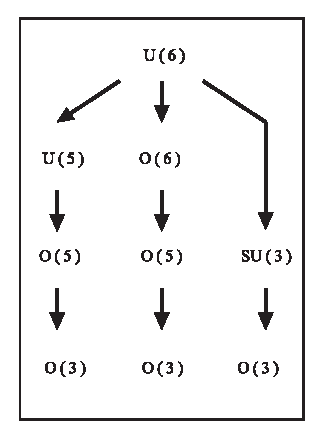
\includegraphics[scale=.65]{figure}
%
% If not, use
%\picplace{5cm}{2cm} % Give the correct figure height and width in cm
%
\caption{If the width of the figure is less than 7.8 cm use the \texttt{sidecapion} command to flush the caption on the left side of the page. If the figure is positioned at the top of the page, align the sidecaption with the top of the figure -- to achieve this you simply need to use the optional argument \texttt{[t]} with the \texttt{sidecaption} command}
\label{fig:1}       % Give a unique label
\end{figure}


\paragraph{Paragraph Heading} %
Instead of simply listing headings of different levels we recommend to let every heading be followed by at least a short passage of text. Furtheron please use the \LaTeX\ automatism for all your cross-references and citations as has already been described in Sect.~\ref{sec:2}.

Please note that the first line of text that follows a heading is not indented, whereas the first lines of all subsequent paragraphs are.

For typesetting numbered lists we recommend to use the \verb|enumerate| environment -- it will automatically render Springer's preferred layout.

\begin{enumerate}
\item{Livelihood and survival mobility are oftentimes coutcomes of uneven socioeconomic development.}
\begin{enumerate}
\item{Livelihood and survival mobility are oftentimes coutcomes of uneven socioeconomic development.}
\item{Livelihood and survival mobility are oftentimes coutcomes of uneven socioeconomic development.}
\end{enumerate}
\item{Livelihood and survival mobility are oftentimes coutcomes of uneven socioeconomic development.}
\end{enumerate}


\subparagraph{Subparagraph Heading} In order to avoid simply listing headings of different levels we recommend to let every heading be followed by at least a short passage of text. Use the \LaTeX\ automatism for all your cross-references and citations as has already been described in Sect.~\ref{sec:2}, see also Fig.~\ref{fig:2}.

Please note that the first line of text that follows a heading is not indented, whereas the first lines of all subsequent paragraphs are.

For unnumbered list we recommend to use the \verb|itemize| environment -- it will automatically render Springer's preferred layout.

\begin{itemize}
\item{Livelihood and survival mobility are oftentimes coutcomes of uneven socioeconomic development, cf. Table~\ref{tab:1}.}
\begin{itemize}
\item{Livelihood and survival mobility are oftentimes coutcomes of uneven socioeconomic development.}
\item{Livelihood and survival mobility are oftentimes coutcomes of uneven socioeconomic development.}
\end{itemize}
\item{Livelihood and survival mobility are oftentimes coutcomes of uneven socioeconomic development.}
\end{itemize}

\begin{figure}[t]
\sidecaption[t]
% Use the relevant command for your figure-insertion program
% to insert the figure file.
% For example, with the option graphics use
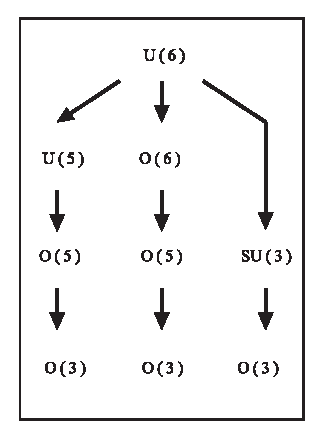
\includegraphics[scale=.65]{figure}
%
% If not, use
%\picplace{5cm}{2cm} % Give the correct figure height and width in cm
%
\caption{Please write your figure caption here}
\label{fig:2}       % Give a unique label
\end{figure}

\runinhead{Run-in Heading Boldface Version} Use the \LaTeX\ automatism for all your cross-references and citations as has already been described in Sect.~\ref{sec:2}.

\subruninhead{Run-in Heading Boldface and Italic Version} Use the \LaTeX\ automatism for all your cross-refer\-ences and citations as has already been described in Sect.~\ref{sec:2}\index{paragraph}.

\subsubruninhead{Run-in Heading Displayed Version} Use the \LaTeX\ automatism for all your cross-refer\-ences and citations as has already been described in Sect.~\ref{sec:2}\index{paragraph}.
% Use the \index{} command to code your index words
%
% For tables use
%
\begin{table}[!t]
\caption{Please write your table caption here}
\label{tab:1}       % Give a unique label
%
% For LaTeX tables use
%
\begin{tabular}{p{2cm}p{2.4cm}p{2cm}p{4.9cm}}
\hline\noalign{\smallskip}
Classes & Subclass & Length & Action Mechanism  \\
\noalign{\smallskip}\svhline\noalign{\smallskip}
Translation & mRNA$^a$  & 22 (19--25) & Translation repression, mRNA cleavage\\
Translation & mRNA cleavage & 21 & mRNA cleavage\\
Translation & mRNA  & 21--22 & mRNA cleavage\\
Translation & mRNA  & 24--26 & Histone and DNA Modification\\
\noalign{\smallskip}\hline\noalign{\smallskip}
\end{tabular}
$^a$ Table foot note (with superscript)
\end{table}
%
\section{Section Heading}
\label{sec:3}
% Always give a unique label
% and use \ref{<label>} for cross-references
% and \cite{<label>} for bibliographic references
% use \sectionmark{}
% to alter or adjust the section heading in the running head
Instead of simply listing headings of different levels we recommend to let every heading be followed by at least a short passage of text. Furtheron please use the \LaTeX\ automatism for all your cross-references and citations as has already been described in Sect.~\ref{sec:2}.

Please note that the first line of text that follows a heading is not indented, whereas the first lines of all subsequent paragraphs are.

If you want to list definitions or the like we recommend to use the Springer-enhanced \verb|description| environment -- it will automatically render Springer's preferred layout.

\begin{description}[Type 1]
\item[Type 1]{That addresses central themes pertainng to migration, health, and disease. In Sect.~\ref{sec:1}, Wilson discusses the role of human migration in infectious disease distributions and patterns.}
\item[Type 2]{That addresses central themes pertainng to migration, health, and disease. In Sect.~\ref{subsec:2}, Wilson discusses the role of human migration in infectious disease distributions and patterns.}
\end{description}

\subsection{Subsection Heading} %
In order to avoid simply listing headings of different levels we recommend to let every heading be followed by at least a short passage of text. Use the \LaTeX\ automatism for all your cross-references and citations citations as has already been described in Sect.~\ref{sec:2}.

Please note that the first line of text that follows a heading is not indented, whereas the first lines of all subsequent paragraphs are.

\begin{svgraybox}
If you want to emphasize complete paragraphs of texts we recommend to use the newly defined Springer class option \verb|graybox| and the newly defined environment \verb|svgraybox|. This will produce a 15 percent screened box 'behind' your text.

If you want to emphasize complete paragraphs of texts we recommend to use the newly defined Springer class option and environment \verb|svgraybox|. This will produce a 15 percent screened box 'behind' your text.
\end{svgraybox}


\subsubsection{Subsubsection Heading}
Instead of simply listing headings of different levels we recommend to let every heading be followed by at least a short passage of text. Furtheron please use the \LaTeX\ automatism for all your cross-references and citations as has already been described in Sect.~\ref{sec:2}.

Please note that the first line of text that follows a heading is not indented, whereas the first lines of all subsequent paragraphs are.

\begin{theorem}
Theorem text goes here.
\end{theorem}
%
% or
%
\begin{definition}
Definition text goes here.
\end{definition}

\begin{proof}
%\smartqed
Proof text goes here.
%\qed
\end{proof}

\paragraph{Paragraph Heading} %
Instead of simply listing headings of different levels we recommend to let every heading be followed by at least a short passage of text. Furtheron please use the \LaTeX\ automatism for all your cross-references and citations as has already been described in Sect.~\ref{sec:2}.

Note that the first line of text that follows a heading is not indented, whereas the first lines of all subsequent paragraphs are.
%
% For built-in environments use
%
\begin{theorem}
Theorem text goes here.
\end{theorem}
%
\begin{definition}
Definition text goes here.
\end{definition}
%
\begin{proof}
%\smartqed
Proof text goes here.
%\qed
\end{proof}
%
%
\begin{trailer}{Trailer Head}
If you want to emphasize complete paragraphs of texts in an \verb|Trailer Head| we recommend to
use  \begin{verbatim}\begin{trailer}{Trailer Head}
...
\end{trailer}\end{verbatim}
\end{trailer}
%
\begin{question}{Questions}
If you want to emphasize complete paragraphs of texts in an \verb|Questions| we recommend to
use  \begin{verbatim}\begin{question}{Questions}
...
\end{question}\end{verbatim}
\end{question}
%
%
\begin{important}{Important}
If you want to emphasize complete paragraphs of texts in an \verb|Important| we recommend to
use  \begin{verbatim}\begin{important}{Important}
...
\end{important}\end{verbatim}
\end{important}
%
\clearpage
\begin{warning}{Attention}
If you want to emphasize complete paragraphs of texts in an \verb|Attention| we recommend to
use  \begin{verbatim}\begin{warning}{Attention}
...
\end{warning}\end{verbatim}
\end{warning}

\begin{programcode}{Program Code}
If you want to emphasize complete paragraphs of texts in an \verb|Program Code| we recommend to
use

\verb|\begin{programcode}{Program Code}|

\verb|\begin{verbatim}...\end{verbatim}|

\verb|\end{programcode}|

\end{programcode}
%
\begin{tips}{Tips}
If you want to emphasize complete paragraphs of texts in an \verb|Tips| we recommend to
use  \begin{verbatim}\begin{tips}{Tips}
...
\end{tips}\end{verbatim}
\end{tips}
%
%
\begin{overview}{Overview}
If you want to emphasize complete paragraphs of texts in an \verb|Overview| we recommend to
use  \begin{verbatim}\begin{overview}{Overview}
...
\end{overview}\end{verbatim}
\end{overview}
\clearpage
\begin{backgroundinformation}{Background Information}
If you want to emphasize complete paragraphs of texts in an \verb|Background|
\verb|Information| we recommend to
use

\verb|\begin{backgroundinformation}{Background Information}|

\verb|...|

\verb|\end{backgroundinformation}|
\end{backgroundinformation}
\begin{legaltext}{Legal Text}
If you want to emphasize complete paragraphs of texts in an \verb|Legal Text| we recommend to
use  \begin{verbatim}\begin{legaltext}{Legal Text}
...
\end{legaltext}\end{verbatim}
\end{legaltext}
%
\begin{acknowledgement}
If you want to include acknowledgments of assistance and the like at the end of an individual chapter please use the \verb|acknowledgement| environment -- it will automatically render Springer's preferred layout.
\end{acknowledgement}
%
\section*{Appendix}
\addcontentsline{toc}{section}{Appendix}
%
When placed at the end of a chapter or contribution (as opposed to at the end of the book), the numbering of tables, figures, and equations in the appendix section continues on from that in the main text. Hence please \textit{do not} use the \verb|appendix| command when writing an appendix at the end of your chapter or contribution. If there is only one the appendix is designated ``Appendix'', or ``Appendix 1'', or ``Appendix 2'', etc. if there is more than one.

\begin{equation}
a \times b = c
\end{equation}
% Problems or Exercises should be sorted chapterwise
\section*{Problems}
\addcontentsline{toc}{section}{Problems}
%
% Use the following environment.
% Don't forget to label each problem;
% the label is needed for the solutions' environment
\begin{prob}
\label{prob1}
A given problem or Excercise is described here. The
problem is described here. The problem is described here.
\end{prob}

\begin{prob}
\label{prob2}
\textbf{Problem Heading}\\
(a) The first part of the problem is described here.\\
(b) The second part of the problem is described here.
\end{prob}

%%%%%%%%%%%%%%%%%%%%%%%% referenc.tex %%%%%%%%%%%%%%%%%%%%%%%%%%%%%%
% sample references
% %
% Use this file as a template for your own input.
%
%%%%%%%%%%%%%%%%%%%%%%%% Springer-Verlag %%%%%%%%%%%%%%%%%%%%%%%%%%
%
% BibTeX users please use
% \bibliographystyle{}
% \bibliography{}
%
\biblstarthook{In view of the parallel print and (chapter-wise) online publication of your book at \url{www.springerlink.com} it has been decided that -- as a genreral rule --  references should be sorted chapter-wise and placed at the end of the individual chapters. However, upon agreement with your contact at Springer you may list your references in a single seperate chapter at the end of your book. Deactivate the class option \texttt{sectrefs} and the \texttt{thebibliography} environment will be put out as a chapter of its own.\\\indent
References may be \textit{cited} in the text either by number (preferred) or by author/year.\footnote{Make sure that all references from the list are cited in the text. Those not cited should be moved to a separate \textit{Further Reading} section or chapter.} If the citatiion in the text is numbered, the reference list should be arranged in ascending order. If the citation in the text is author/year, the reference list should be \textit{sorted} alphabetically and if there are several works by the same author, the following order should be used:
\begin{enumerate}
\item all works by the author alone, ordered chronologically by year of publication
\item all works by the author with a coauthor, ordered alphabetically by coauthor
\item all works by the author with several coauthors, ordered chronologically by year of publication.
\end{enumerate}
The \textit{styling} of references\footnote{Always use the standard abbreviation of a journal's name according to the ISSN \textit{List of Title Word Abbreviations}, see \url{http://www.issn.org/en/node/344}} depends on the subject of your book:
\begin{itemize}
\item The \textit{two} recommended styles for references in books on \textit{mathematical, physical, statistical and computer sciences} are depicted in ~\cite{science-contrib, science-online, science-mono, science-journal, science-DOI} and ~\cite{phys-online, phys-mono, phys-journal, phys-DOI, phys-contrib}.
\item Examples of the most commonly used reference style in books on \textit{Psychology, Social Sciences} are~\cite{psysoc-mono, psysoc-online,psysoc-journal, psysoc-contrib, psysoc-DOI}.
\item Examples for references in books on \textit{Humanities, Linguistics, Philosophy} are~\cite{humlinphil-journal, humlinphil-contrib, humlinphil-mono, humlinphil-online, humlinphil-DOI}.
\item Examples of the basic Springer style used in publications on a wide range of subjects such as \textit{Computer Science, Economics, Engineering, Geosciences, Life Sciences, Medicine, Biomedicine} are ~\cite{basic-contrib, basic-online, basic-journal, basic-DOI, basic-mono}. 
\end{itemize}
}

\begin{thebibliography}{99.}%
% and use \bibitem to create references.
%
% Use the following syntax and markup for your references if 
% the subject of your book is from the field 
% "Mathematics, Physics, Statistics, Computer Science"
%
% Contribution 
\bibitem{science-contrib} Broy, M.: Software engineering --- from auxiliary to key technologies. In: Broy, M., Dener, E. (eds.) Software Pioneers, pp. 10-13. Springer, Heidelberg (2002)
%
% Online Document
\bibitem{science-online} Dod, J.: Effective substances. In: The Dictionary of Substances and Their Effects. Royal Society of Chemistry (1999) Available via DIALOG. \\
\url{http://www.rsc.org/dose/title of subordinate document. Cited 15 Jan 1999}
%
% Monograph
\bibitem{science-mono} Geddes, K.O., Czapor, S.R., Labahn, G.: Algorithms for Computer Algebra. Kluwer, Boston (1992) 
%
% Journal article
\bibitem{science-journal} Hamburger, C.: Quasimonotonicity, regularity and duality for nonlinear systems of partial differential equations. Ann. Mat. Pura. Appl. \textbf{169}, 321--354 (1995)
%
% Journal article by DOI
\bibitem{science-DOI} Slifka, M.K., Whitton, J.L.: Clinical implications of dysregulated cytokine production. J. Mol. Med. (2000) doi: 10.1007/s001090000086 
%
\bigskip

% Use the following (APS) syntax and markup for your references if 
% the subject of your book is from the field 
% "Mathematics, Physics, Statistics, Computer Science"
%
% Online Document
\bibitem{phys-online} J. Dod, in \textit{The Dictionary of Substances and Their Effects}, Royal Society of Chemistry. (Available via DIALOG, 1999), 
\url{http://www.rsc.org/dose/title of subordinate document. Cited 15 Jan 1999}
%
% Monograph
\bibitem{phys-mono} H. Ibach, H. L\"uth, \textit{Solid-State Physics}, 2nd edn. (Springer, New York, 1996), pp. 45-56 
%
% Journal article
\bibitem{phys-journal} S. Preuss, A. Demchuk Jr., M. Stuke, Appl. Phys. A \textbf{61}
%
% Journal article by DOI
\bibitem{phys-DOI} M.K. Slifka, J.L. Whitton, J. Mol. Med., doi: 10.1007/s001090000086
%
% Contribution 
\bibitem{phys-contrib} S.E. Smith, in \textit{Neuromuscular Junction}, ed. by E. Zaimis. Handbook of Experimental Pharmacology, vol 42 (Springer, Heidelberg, 1976), p. 593
%
\bigskip
%
% Use the following syntax and markup for your references if 
% the subject of your book is from the field 
% "Psychology, Social Sciences"
%
%
% Monograph
\bibitem{psysoc-mono} Calfee, R.~C., \& Valencia, R.~R. (1991). \textit{APA guide to preparing manuscripts for journal publication.} Washington, DC: American Psychological Association.
%
% Online Document
\bibitem{psysoc-online} Dod, J. (1999). Effective substances. In: The dictionary of substances and their effects. Royal Society of Chemistry. Available via DIALOG. \\
\url{http://www.rsc.org/dose/Effective substances.} Cited 15 Jan 1999.
%
% Journal article
\bibitem{psysoc-journal} Harris, M., Karper, E., Stacks, G., Hoffman, D., DeNiro, R., Cruz, P., et al. (2001). Writing labs and the Hollywood connection. \textit{J Film} Writing, 44(3), 213--245.
%
% Contribution 
\bibitem{psysoc-contrib} O'Neil, J.~M., \& Egan, J. (1992). Men's and women's gender role journeys: Metaphor for healing, transition, and transformation. In B.~R. Wainrig (Ed.), \textit{Gender issues across the life cycle} (pp. 107--123). New York: Springer.
%
% Journal article by DOI
\bibitem{psysoc-DOI}Kreger, M., Brindis, C.D., Manuel, D.M., Sassoubre, L. (2007). Lessons learned in systems change initiatives: benchmarks and indicators. \textit{American Journal of Community Psychology}, doi: 10.1007/s10464-007-9108-14.
%
%
% Use the following syntax and markup for your references if 
% the subject of your book is from the field 
% "Humanities, Linguistics, Philosophy"
%
\bigskip
%
% Journal article
\bibitem{humlinphil-journal} Alber John, Daniel C. O'Connell, and Sabine Kowal. 2002. Personal perspective in TV interviews. \textit{Pragmatics} 12:257--271
%
% Contribution 
\bibitem{humlinphil-contrib} Cameron, Deborah. 1997. Theoretical debates in feminist linguistics: Questions of sex and gender. In \textit{Gender and discourse}, ed. Ruth Wodak, 99--119. London: Sage Publications.
%
% Monograph
\bibitem{humlinphil-mono} Cameron, Deborah. 1985. \textit{Feminism and linguistic theory.} New York: St. Martin's Press.
%
% Online Document
\bibitem{humlinphil-online} Dod, Jake. 1999. Effective substances. In: The dictionary of substances and their effects. Royal Society of Chemistry. Available via DIALOG. \\
http://www.rsc.org/dose/title of subordinate document. Cited 15 Jan 1999
%
% Journal article by DOI
\bibitem{humlinphil-DOI} Suleiman, Camelia, Daniel C. O'Connell, and Sabine Kowal. 2002. `If you and I, if we, in this later day, lose that sacred fire...': Perspective in political interviews. \textit{Journal of Psycholinguistic Research}. doi: 10.1023/A:1015592129296.
%
%
%
\bigskip
%
%
% Use the following syntax and markup for your references if 
% the subject of your book is from the field 
% "Computer Science, Economics, Engineering, Geosciences, Life Sciences"
%
%
% Contribution 
\bibitem{basic-contrib} Brown B, Aaron M (2001) The politics of nature. In: Smith J (ed) The rise of modern genomics, 3rd edn. Wiley, New York 
%
% Online Document
\bibitem{basic-online} Dod J (1999) Effective Substances. In: The dictionary of substances and their effects. Royal Society of Chemistry. Available via DIALOG. \\
\url{http://www.rsc.org/dose/title of subordinate document. Cited 15 Jan 1999}
%
% Journal article by DOI
\bibitem{basic-DOI} Slifka MK, Whitton JL (2000) Clinical implications of dysregulated cytokine production. J Mol Med, doi: 10.1007/s001090000086
%
% Journal article
\bibitem{basic-journal} Smith J, Jones M Jr, Houghton L et al (1999) Future of health insurance. N Engl J Med 965:325--329
%
% Monograph
\bibitem{basic-mono} South J, Blass B (2001) The future of modern genomics. Blackwell, London 
%
\end{thebibliography}


%%%%%%%%%%%%%%%%%%%%%% appendix.tex %%%%%%%%%%%%%%%%%%%%%%%%%%%%%%%%%
%
% sample appendix
%
% Use this file as a template for your own input.
%
%%%%%%%%%%%%%%%%%%%%%%%% Springer-Verlag %%%%%%%%%%%%%%%%%%%%%%%%%%

\appendix
\motto{All's well that ends well}
\chapter{Chapter Heading}
\label{introA} % Always give a unique label
% use \chaptermark{}
% to alter or adjust the chapter heading in the running head

Use the template \emph{appendix.tex} together with the Springer document class SVMono (monograph-type books) or SVMult (edited books) to style appendix of your book.


\section{Section Heading}
\label{sec:A1}
% Always give a unique label
% and use \ref{<label>} for cross-references
% and \cite{<label>} for bibliographic references
% use \sectionmark{}
% to alter or adjust the section heading in the running head
Instead of simply listing headings of different levels we recommend to let every heading be followed by at least a short passage of text. Furtheron please use the \LaTeX\ automatism for all your cross-references and citations.


\subsection{Subsection Heading}
\label{sec:A2}
Instead of simply listing headings of different levels we recommend to let every heading be followed by at least a short passage of text. Furtheron please use the \LaTeX\ automatism for all your cross-references and citations as has already been described in Sect.~\ref{sec:A1}.

For multiline equations we recommend to use the \verb|eqnarray| environment.
\begin{eqnarray}
\vec{a}\times\vec{b}=\vec{c} \nonumber\\
\vec{a}\times\vec{b}=\vec{c}
\label{eq:A01}
\end{eqnarray}

\subsubsection{Subsubsection Heading}
Instead of simply listing headings of different levels we recommend to let every heading be followed by at least a short passage of text. Furtheron please use the \LaTeX\ automatism for all your cross-references and citations as has already been described in Sect.~\ref{sec:A2}.

Please note that the first line of text that follows a heading is not indented, whereas the first lines of all subsequent paragraphs are.

% For figures use
%
\begin{figure}[t]
\sidecaption[t]
%\centering
% Use the relevant command for your figure-insertion program
% to insert the figure file.
% For example, with the option graphics use
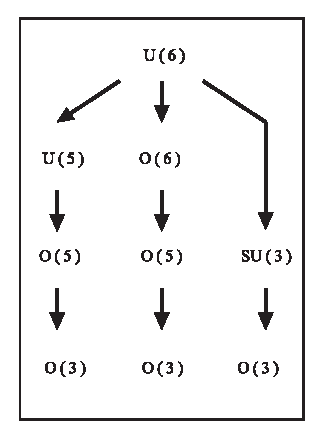
\includegraphics[scale=.65]{figure}
%
% If not, use
%\picplace{5cm}{2cm} % Give the correct figure height and width in cm
%
\caption{Please write your figure caption here}
\label{fig:A1}       % Give a unique label
\end{figure}

% For tables use
%
\begin{table}
\caption{Please write your table caption here}
\label{tab:A1}       % Give a unique label
%
% For LaTeX tables use
%
\begin{tabular}{p{2cm}p{2.4cm}p{2cm}p{4.9cm}}
\hline\noalign{\smallskip}
Classes & Subclass & Length & Action Mechanism  \\
\noalign{\smallskip}\hline\noalign{\smallskip}
Translation & mRNA$^a$  & 22 (19--25) & Translation repression, mRNA cleavage\\
Translation & mRNA cleavage & 21 & mRNA cleavage\\
Translation & mRNA  & 21--22 & mRNA cleavage\\
Translation & mRNA  & 24--26 & Histone and DNA Modification\\
\noalign{\smallskip}\hline\noalign{\smallskip}
\end{tabular}
$^a$ Table foot note (with superscript)
\end{table}
%


\backmatter%%%%%%%%%%%%%%%%%%%%%%%%%%%%%%%%%%%%%%%%%%%%%%%%%%%%%%%
\clearpage
\addcontentsline{toc}{chapter}{Bibliography}
\bibliographystyle{plain}
\bibliography{references}

\clearpage
\addcontentsline{toc}{chapter}{Index}
%%%%%%%%%%%%%%%%%%%%%%%acronym.tex%%%%%%%%%%%%%%%%%%%%%%%%%%%%%%%%%%%%%%%%%
% sample list of acronyms
%
% Use this file as a template for your own input.
%
%%%%%%%%%%%%%%%%%%%%%%%% Springer %%%%%%%%%%%%%%%%%%%%%%%%%%

\Extrachap{Glossary}


Use the template \emph{glossary.tex} together with the Springer document class SVMono (monograph-type books) or SVMult (edited books) to style your glossary\index{glossary} in the Springer layout.


\runinhead{glossary term} Write here the description of the glossary term. Write here the description of the glossary term. Write here the description of the glossary term.

\runinhead{glossary term} Write here the description of the glossary term. Write here the description of the glossary term. Write here the description of the glossary term.

\runinhead{glossary term} Write here the description of the glossary term. Write here the description of the glossary term. Write here the description of the glossary term.

\runinhead{glossary term} Write here the description of the glossary term. Write here the description of the glossary term. Write here the description of the glossary term.

\runinhead{glossary term} Write here the description of the glossary term. Write here the description of the glossary term. Write here the description of the glossary term.
%
\Extrachap{Solutions}

\section*{Problems of Chapter~\ref{intro}}

\begin{sol}{prob1}
The solution\index{problems}\index{solutions} is revealed here.
\end{sol}


\begin{sol}{prob2}
\textbf{Problem Heading}\\
(a) The solution of first part is revealed here.\\
(b) The solution of second part is revealed here.
\end{sol}


\printindex

%%%%%%%%%%%%%%%%%%%%%%%%%%%%%%%%%%%%%%%%%%%%%%%%%%%%%%%%%%%%%%%%%%%%%%

\end{document}





